%!TEX root = ../template.tex
%%%%%%%%%%%%%%%%%%%%%%%%%%%%%%%%%%%%%%%%%%%%%%%%%%%%%%%%%%%%%%%%%%%
%% chapter1.tex
%% NOVA thesis document file
%%
%% Chapter with introduction
%%%%%%%%%%%%%%%%%%%%%%%%%%%%%%%%%%%%%%%%%%%%%%%%%%%%%%%%%%%%%%%%%%%

\typeout{NT FILE state_of_the_art.tex}%

\chapter{State of the Art}
\label{cha:state_of_the_art}

% \prependtographicspath{{Chapters/Figures/Covers/}}

% epigraph configuration
\epigraphfontsize{\small\itshape}
\setlength\epigraphwidth{12.5cm}
\setlength\epigraphrule{0pt}


In this chapter we'll present our state of the art research. We performed a short Manual Search and a Systematic Mapping Study (SMS).


%%%%%%%%%%%%%%%%%%%%%%%%%%%%%%%%%%%%%%%%%%%%%
%%%%%%%%%%%%%%% MANUAL SEARCH %%%%%%%%%%%%%%%
%%%%%%%%%%%%%%%%%%%%%%%%%%%%%%%%%%%%%%%%%%%%%

\section{Manual Search}
I this chapter we'll go over the manual research conducted, where we review relevant literature. We begin by examining articles related to existing approaches for requirements elicitation.
As well as existing apporaches for ethical requirements elicitation. We also analyze articles related to the usage of AI to gather requirements. Lastly, we'll discuss the recent advancements in
using LLMs for ethical requirements elicitation, highlighting their potential and limitations. 
  

\subsection{Card-Based and Catalog Approaches}
This subsection covers methods that use modular tools (cards, catalogs) to support the elicitation process.

The approach outlined in \cite{halme2021write} is the ECCOLA method \cite{VAKKURI2021111067}, which is designed to help developers integrate AI ethics into the development of AI systems. This method offers a practical, 
modular, and sprint-based framework that fits within agile development practices. ECCOLA consists of 21 cards organized into 9 themes, including Transparency, Fairness, and Accountability. 
Each card describes an ethical issue, suggests actions that developers can take, and provides real-world examples. 
At the beginning of each sprint, developers select the relevant cards, use them during development, and document their ethical considerations. However, it is important to note that ECCOLA was 
specifically designed for AI and autonomous systems, so it may not be the most suitable approach for projects that do not focus on AI. Additionally, the card-based system requires training and 
familiarization, meaning teams must invest time in learning how to use the cards and incorporating them into their workflow.
Furthermore, this approach does not provide straightforward answers but instead serves as a framework to encourage discussion and reflection on ethical issues throughout the development process.
Additionally, many users preferred to use ECCOLA's cards selectively, tailoring them to their immediate needs instead of repeating the full process as instructed. 
While this modular approach allows for flexibility, it risks missing critical ethical dimensions by not exhaustively addressing all possibilities in each iteration.

In the study \cite{ahmad2023requirements}, the authors introduced the RE4HCAI (Requirements Engineering for Human-Centered AI) framework, which emphasizes the integration of human-centered principles in requirements 
engineering (RE) for AI-based software. Traditional AI development often overlooks critical aspects such as ethics, bias, inclusivity, and user needs, which can lead to the creation of non-inclusive and biased systems 
\cite{buolamwini2018gender}. 
The proposed framework aligns with existing industrial guidelines from companies like Google\footnote{Google AI Principles: \url{https://ai.google/responsibility/principles/}} and Microsoft\footnote{Microsoft Responsible AI: \url{https://learn.microsoft.com/en-us/azure/machine-learning/concept-responsible-ai}}, 
incorporating insights from systematic literature reviews (SLRs) and expert surveys. It utilizes a conceptual model that organizes the requirements process into key human-centered areas: user needs, 
model needs, data needs, feedback and user control, explainability and trust, and errors and failures. To support these areas, the authors developed a catalog to assist in eliciting and modeling 
requirements. The RE4HCAI framework consists of three layers: human-centered guidelines mapped into a reference model; a catalog for detailed requirements elicitation; and a modeling language with 
visual notations for presenting requirements. This framework enhances the understanding of human-centered requirements and underscores the iterative nature of RE for AI-based software, which requires 
continuous evaluation of user and system needs. Feedback from the study indicated that integrating human-centered values into RE improves inclusivity and reduces biases. However, the approach primarily 
provides a catalog focused on AI-based software requirements. This reliance on a static catalog may not address the dynamic nature of ethical challenges in the field. Additionally, its emphasis on AI 
may limit its applicability to other domains, raising concerns about subjectivity and a lack of broad empirical validation.


\subsection{Agile Techniques: Ethical User Stories}
In agile contexts, translating ethical principles into actionable user stories can bridge the gap between abstract guidelines and development tasks.

In this study \cite{halme2024making}, the authors introduce "Ethical User Stories" (EUSs), a novel approach that integrates ethical considerations into the agile requirements engineering process. 
This method translates abstract ethical principles into actionable, concrete requirements. EUSs empower developers, even those without extensive backgrounds in ethics, to incorporate ethical 
considerations into their work. Developed through three iterations of design science research (DSR) and involving 659 user stories, this approach shows promise in bridging the gap between abstract 
ethical principles and their practical implementation in SE.
The process of creating an EUS involves four main steps. First, there needs to be a motivation for developing an ethical system, which may arise from customer concerns or stakeholder priorities. 
Additionally, the type of system being developed must be considered. Next, an appropriate ethical framework should be selected. This framework may consist of guidelines, a method, or even an 
ethical theory, but it must be relevant to the product being developed.
After selecting the framework, ethical user stories can be created. These stories adhere to the same structure as traditional user stories: "As a <role>, I want to <goal>, so that <reason>." 
However, they must include an ethical reference that connects the story to the chosen ethical framework. The user stories should address the ethical issues identified through the framework. 
Finally, these ethical user stories are utilized to determine both functional and non-functional requirements for the system.
The success of EUSs, however, hinges on having a suitable ethical framework to define issues and guide discussions.


%%%%%%%%%%%%%%%%%%%%%%%%%%%%%%%%%%%%%%%%%%%%%%%%%%%%%%%%%%%%%%%%%%%%%%
% AI-Assisted Approaches for Requirements Elicitation
%%%%%%%%%%%%%%%%%%%%%%%%%%%%%%%%%%%%%%%%%%%%%%%%%%%%%%%%%%%%%%%%%%%%%%
\subsection{AI-Assisted Approaches for Requirements Elicitation}
Recent advances in AI have paved the way for techniques that augment traditional elicitation methods. This section discusses approaches where AI is used to discover requirements more efficiently.

\subsubsection{Agent-Based Simulation}
The study in \cite{ataei2024elicitron} introduces a new approach that utilizes LLMs to enhance and partially automate RE. These models can 
simulate user interactions and perspectives to identify a broader range of needs, including latent or unarticulated ones.
The research presents a framework called Elicitron, which employs LLMs to generate diverse user agents capable of role-playing in product experience scenarios. These agents produce structured 
outputs that are highly relevant to the RE process, enabling the discovery of needs that traditional methods may struggle to capture. This approach also allows for scalability; experiments 
demonstrate its effectiveness in generating both diverse and latent needs, often outperforming human interviews in this regard.
While LLMs have potential drawbacks, such as a tendency to predict the most likely outcomes, the research argues that careful contextualization can guide them to generate outputs that assist 
designers in uncovering a broader range of user needs. The study also highlights the effectiveness of LLMs in analyzing interview data and classifying needs.
However, this method mainly focuses on identifying design requirements, particularly latent needs, which can be non-obvious and only recognized in later stages of development. These types of 
requirements differ from ethical requirements, as they primarily concern the usability of the product under development. Nevertheless, with the recent advancements in LLMs and AI, a similar 
process could also be useful for identifying ethical requirements.

The authors in \cite{zhang2024llm} investigate the potential of LLMs to automate user story refinement through an Autonomous LLM-based Agent System (ALAS). ALAS aims to enhance 
requirements management within agile environments. It functions through AI agents that simulate agile roles and facilitate collaborative interactions.
The task prompts were designed to mimic real project contexts. Initial prompts defined the agent's role, the task, and its context, while follow-up prompts guided subsequent subtasks. Two primary agent profiles were 
established—Product Owner (PO) and Requirements Engineer—each responsible for different aspects of user story quality. The agents utilized contextual documents, such as a Minimum Viable Product (MVP) outline and a 
product vision statement, to ensure alignment with project goals.
After the experimentation phase, feedback from participants, which included experienced team members from six agile teams, indicated that while ALAS improved story coherence, additional input from POs and domain experts 
is necessary to avoid irrelevant out-of-scope details and to refine prompts for greater project-specific relevance. The study also observed that although adjusting the "Temperature" parameter of the model encouraged 
creativity, it could result in plausible yet irrelevant outputs. Hence, employing techniques like retrieval-augmented generation (RAG) may help maintain accuracy.
In conclusion, while this method is not directly related to eliciting ethical requirements, its approach is quite similar to previously established methods for ethical requirements elicitation.



%%%%%%%%%%%%%%%%%%%%%%%%%%%%%%%%%%%%%%%%%%%%%%%%%%%%%%%%
%%%%%%%%%%%%%%% SYSTEMATIC MAPPING STUDY %%%%%%%%%%%%%%%
%%%%%%%%%%%%%%%%%%%%%%%%%%%%%%%%%%%%%%%%%%%%%%%%%%%%%%%%

\section{Systematic Mapping Study}
\label{sec: SMS}
In this section we'll discuss the performed SMS and the process followed to conduct it as well as our results. We used the study in \cite{bombonatti2016usability} 
to guide and structure and our state of the art research.


% In this section we'll present our Systematic Mapping Study (SMS) and the process followed to conduct it as well as our results. Our objectives with this study is to find the existing approaches
% to elicit ethical requirements.

% We used the study in \cite{bombonatti2016usability} to structure and guide the development of our search string and the Strategy for our SMS. 


\subsection{Search Strategy}
\label{sec: SMS_Search_Strategy}

We plan to answer the research questions (RQs) present in table \ref{tab:research_questions}
\begin{table}[h]
  \centering
  \renewcommand{\arraystretch}{1.3}
  \begin{tabular}{| m{6cm} | m{8cm} |}
      \hline
      \textbf{Research Question} & \textbf{Motivation and Objective} \\
      \hline
      RQ1: Which approaches already exist to specify ethical requirements? & We aim to identify existing approaches to elicit ethical requirements. \\
      \hline
      RQ2: What challenges and limitations do these approaches have? & We aim to have an understanding of the limitations that these approaches face to guide our further research. \\
      \hline
      RQ3: What are the characteristics of these approaches? & We aim to understand how these approaches operate and how they can be relevant to our goal. \\
      \hline
  \end{tabular}
  \caption{Research Questions and Motivations}
  \label{tab:research_questions}
\end{table}

The goal of these questions is to have an unserstanding of the existing approaches to elicit ethical requirements, their limitations and how they function, 
thus having clearer picture of what we can crete or improve upon with this research.

To develop our search string, we conducted several pilot searches to ensure that all terms aligned with our research goals.
The search string is as follows:
\begin{quote}
  \texttt{software AND requirement AND ethics AND elicitation AND (approach OR challenges OR limitations OR characteristics)}
\end{quote} 
It consists of five mandatory terms, \texttt{software}, \texttt{requirement}, \texttt{ethics}, and \texttt{elicitation}, these terms try to guarantee that
our search results are focused in this research topic, and the expression \texttt{(approach OR challenges OR limitations OR characteristics)}, to cover 
the key aspects of our research questions.

\subsubsection{Inclusion and exclusion criteria}
The \textit{inclusion criteria} used were:
\begin{itemize}
  \item Studies published in peer-reviewed journals or presented at reputable conferences.
  \item Studies that address the research questions.
\end{itemize}

As \textit{exclusion criteria} we have:
\begin{itemize}
  \item Studies published before 2016.
  \item Studies not written in English.
  \item Duplicate studies or studies with insufficient methodological rigor.
  \item Secondary or tertiary studies.
\end{itemize}

\subsection{Study Selection}

This search was conducted with the help of Parsifal\footnote{Parsifal: \url{https://parsif.al/}}, a tool used to manage the study selection process and 
record decisions made at each stage. 

The sources for this SMS were the libraries ACM\footnote{ACM: \url{https://dl.acm.org/}}, IEEE\footnote{IEEE: \url{https://ieeexplore.ieee.org/}}, 
ScienceDirect\footnote{ScienceDirect: \url{https://www.sciencedirect.com/}}, and Springer\footnote{ScienceDirect: \url{https://link.springer.com/}}. 
These well-known libraries contain a vast collection of peer-reviewed scientific papers and articles. After applying our inclusion and exclusion 
criteria, we used quality assessment (QA) questions and assigned scores to filter the papers less relevant to our research problem. 
Ultimately, we addressed our research questions (RQs) and excluded studies that did not answer at least one of the RQs.

After applying the search string we retrieved a total of 3,321 papers, 3,887 from ACM, 14 from IEEE, 11,314 from ScienceDirect, and 655 from Springer. 
We then applied different filters for each library:

\begin{itemize}
  \item \textbf{IEEE and ACM}: 
  \begin{itemize}
    \item Years: 2016 - 2025.
  \end{itemize}

  \item \textbf{Springer Link}:  
  \begin{itemize}
    \item Years: 2016 - 2025.
    \item Content type: Chapter, Article, Research article, Conference Paper.
    \item Languages: English.
    \item Subjects: Software engineering, computer ethics, engineering ethics, ethics of technology.
    \item Disciplines: Computer Science.
    \item Subdisciplines: Software engineering/programming and operating systems, software engineering, Computer applications, Programming techniques
  \end{itemize}

  \item \textbf{ScienceDirect}:  
  \begin{itemize}
    \item Years: 2016 - 2025
    \item Article type: Research articles, Book chapters, Practice guidelines, Software publications
    \item Subject areas: Computer Science
  \end{itemize}
\end{itemize}

After applying the filters our study population was trimmed down to more specific works. It resulted in 3,225 studies from ACM, 11 from IEEE, 28 from ScienceDirect, and 57 from Springer.
Since we still had a large ammount of results from the ACM library, we only used to first 50 results ordered by cited plus the first 50 results ordered by recency. So in total 100 results from
the ACM library, gathering 195 studies.

We removed the duplicates using the Parsifal tool, resulting in 193 articles. After applying the inclusion and exclusion criteria we gathered 36 studies. We also used Parsifal for this papers as 
seen in the image \ref{fig:parsifal_accepted_step1}.
A visualization of the study selection process can be seen in figure \ref{fig:study_selection_process}

\begin{figure}[h]
    \centering
    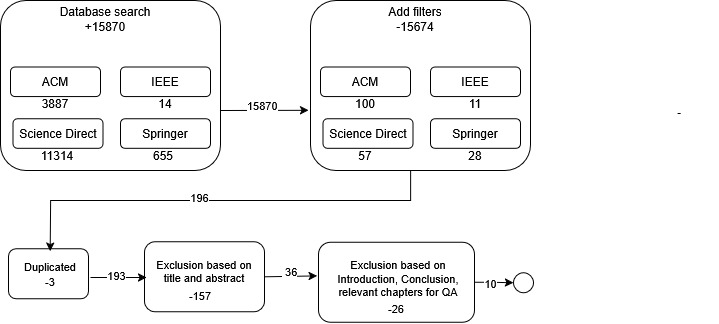
\includegraphics[width=0.8\textwidth]{study_selection_process}
    \caption{Steps for the Study Selection Process}
    \label{fig:study_selection_process}
  \end{figure}

\begin{figure}[h]
  \centering
  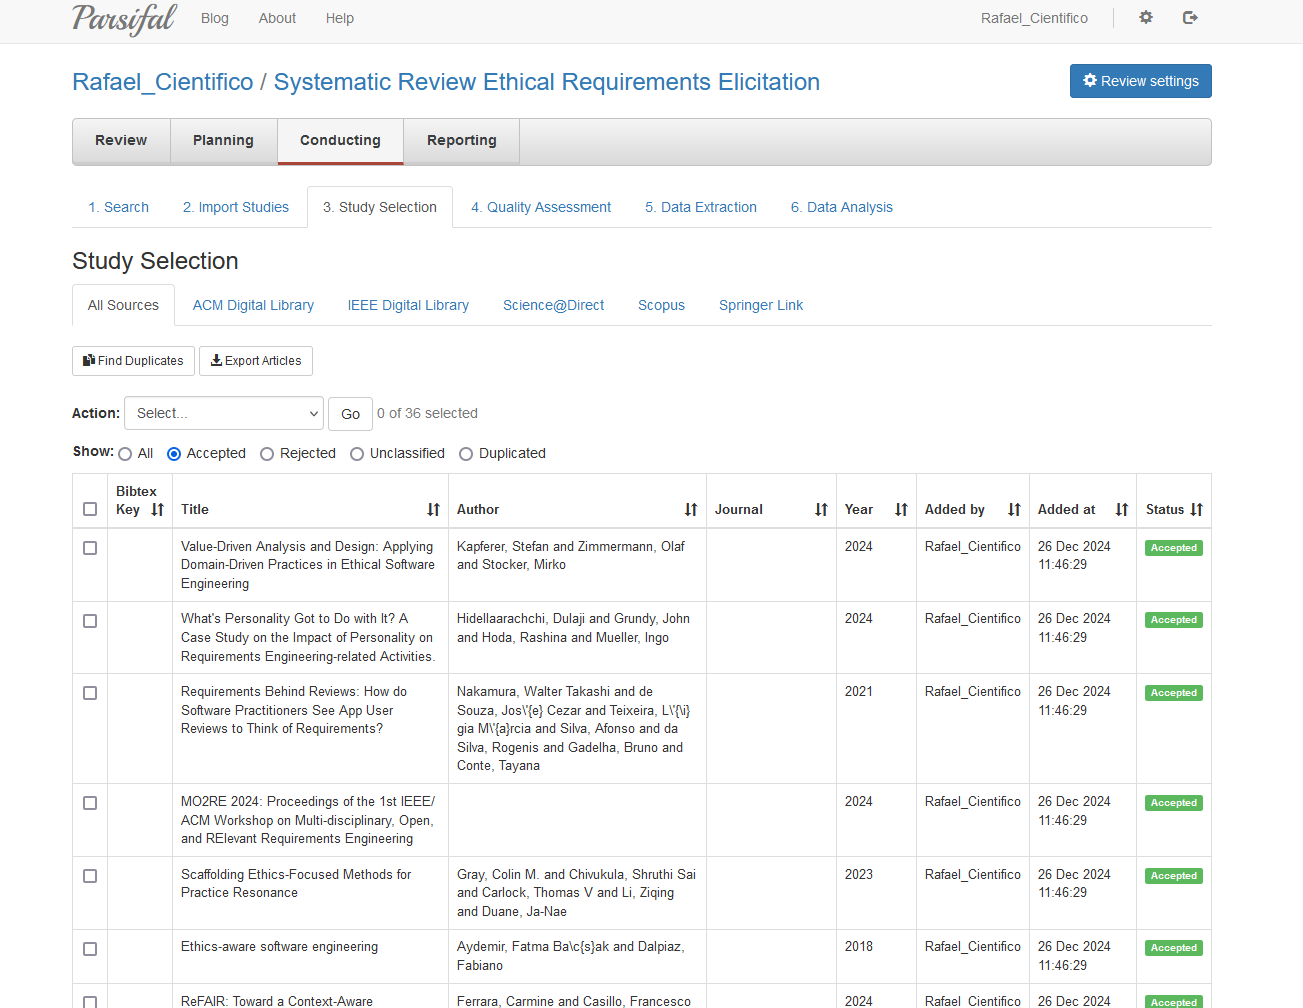
\includegraphics[width=0.8\textwidth]{parsifal_accepted_step1}
  \caption{Accepted Studies after applying inclusion and exclusion criteria}
  \label{fig:parsifal_accepted_step1}
\end{figure}

\subsection{Quality Assessment}
The QA's goal is to measure the level of valuableness of the resulting papers. QA questions are asked to each paper and by reading their introduction, conclusion and relevant chapters, we provide 
an answer. There are three answers available: Yes, Parcially, and No. Each answer with an attributed score, 1, 0.5, 0 respectively. 

All papers were asked the following QA questions:
\begin{itemize}
  \item Did the author presented their difficulties?
  \item Was the solution properly tested?
  \item Is the method clearly explained? 
\end{itemize}

The final quality score for each paper is calculated by summing scores for each question. The scores for each paper can be seen in the table \ref{tab:qa_scoring}

\renewcommand{\arraystretch}{1.1}
\setlength{\tabcolsep}{3pt}
\begin{longtable}{| m{10cm} | m{2cm} |}
    \hline
    \textbf{Paper Title} & \textbf{Quality Score} \\
    \hline
    \endfirsthead
    \hline
    \textbf{Paper Title} & \textbf{Quality Score} \\
    \hline
    \endhead

    IEEE Draft Model Process for Addressing Ethical Concerns During System Design & 0.0 \\
    \hline
    Toolkit for specification, validation and verification of social, legal, ethical, empathetic and cultural requirements for autonomous agents & 1.5 \\
    \hline
    Eliciting Ethicality Requirements Using the Ontology-Based Requirements Engineering Method & 2.5 \\
    \hline
    A Framework for Privacy and Security Requirements Analysis and Conflict Resolution for Supporting GDPR Compliance Through Privacy-by-Design & 0.0 \\
    \hline
    Incorporating Ethical Aspects in Information Systems Requirements Engineering & 0.0 \\
    \hline
    Do You Own a Volkswagen? Values as Non-Functional Requirements & 0.0 \\
    \hline
    Advancing Requirements Engineering Through Generative AI: Assessing the Role of LLMs & 0.0 \\
    \hline
    Value-based requirements engineering: method and experience & 0.0 \\
    \hline
    An ontology-based approach to engineering ethicality requirements & 3.0 \\
    \hline
    Theme section on model-driven requirements engineering & 0.0 \\
    \hline
    Explainable software systems: from requirements analysis to system evaluation & 0.0 \\
    \hline
    The Impact of Personality on Requirements Engineering Activities: A Mixed-Methods Study & 3.0 \\
    \hline
    How mature is requirements engineering for AI-based systems? A systematic mapping study on practices, challenges, and future research directions & 0.0 \\
    \hline
    Using i* to Analyze Ethicality Requirements Following Ontology-Based Requirements Engineering & 0.5 \\
    \hline
    Stakeholder Inclusion and Value Diversity: An Evaluation Using an Access Control System & 0.0 \\
    \hline
    Managing Ethical Requirements Elicitation & 0.0 \\
    \hline
    Trustworthiness Requirements: The Pix Case Study & 2.0 \\
    \hline
    Chapter 12 - Assessing and implementing trustworthy AI across multiple dimensions & 0.5 \\
    \hline
    Requirements engineering for artificial intelligence systems: A systematic mapping study & 0.0 \\
    \hline
    Applying Human Values Theory to Software Engineering Practice: Lessons and Implications & 0.0 \\
    \hline
    IEEE/ISO/IEC International Standard--Systems and software engineering--Life cycle management--Part 7000: Standard model process for addressing ethical concerns during system design & 0.0 \\
    \hline
    IEEE Standard Model Process for Addressing Ethical Concerns during System Design & 0.0 \\
    \hline
    A roadmap for ethics-aware software engineering & 2.0 \\
    \hline
    Teaching Requirements Engineering for AI: A Goal-Oriented Approach in Software Engineering Courses & 2.5 \\
    \hline
    Ethical Requirements Stack: A framework for implementing ethical requirements of AI in software engineering practices & 0.5 \\
    \hline
    Implementing AI Ethics: Making Sense of the Ethical Requirements & 0.0 \\
    \hline
    The Influence of Human Aspects on Requirements Engineering-related Activities: Software Practitioners’ Perspective & 0.5 \\
    \hline
    Interaction design and requirements elicitation integrated through SPIDe: a feasibility study & 3.5 \\
    \hline
    ReFAIR: Toward a Context-Aware Recommender for Fairness Requirements Engineering & 3.5 \\
    \hline
    Ethics-aware software engineering & 0.0 \\
    \hline
    Scaffolding Ethics-Focused Methods for Practice Resonance & 0.0 \\
    \hline
    MO2RE 2024: Proceedings of the 1st IEEE/ACM Workshop on Multi-disciplinary, Open, and RElevant Requirements Engineering & 0.0 \\
    \hline
    Requirements Behind Reviews: How do Software Practitioners See App User Reviews to Think of Requirements? & 0.0 \\
    \hline
    What's Personality Got to Do with It? A Case Study on the Impact of Personality on Requirements Engineering-related Activities. & 0.0 \\
    \hline
    Value-Driven Analysis and Design: Applying Domain-Driven Practices in Ethical Software Engineering & 0.0 \\
    \hline
    The Use of OpenEHR Archetypes in Requirements Elicitation: Best Practices for Engaging Domain Experts in Healthcare Software Development & 2.5 \\
    \hline
    \caption{Scoring of each paper in Quality Assurance phase}
    \label{tab:qa_scoring}
\end{longtable}

Studies with a score below 1 were were excluded.

\subsection{Threats to Validity}
In this section we discuss threats to the validity of our SMS. We followed the guidelines in \cite{montgomery2022empirical}.

% \paragraph{\textbf{Construct validity:}}

% \paragraph{\textbf{Excertal validity:}}

% \paragraph{\textbf{Internal validity:}}


%%%%%%% rever o resto das threats to validity -> nao esta bom %%%%%%%%%%%%%%%%%%%%%%
\paragraph{\textbf{Search String:}}
We developed our search string by experimenting with various query formulations and validating the outcomes. To address our research questions, we incorporated key terms such as "ethics", 
"elicitation", "requirements", "challenges", and "characteristics". Due to ScienceDirect's limitation of allowing only eight Boolean connectors per field, our query was restricted to eight terms. 
Although this approach was intended to limit the number of results for a manageable review, it may have inadvertently excluded some relevant studies.


\paragraph{\textbf{Publication Bias:}}
We initiated our search using four libraries (see Section \ref{sec: SMS_Search_Strategy}), which may have resulted in missing studies available in other databases. 
During our manual search, we discovered additional relevant articles in other sources, such as arXiv\footnote{arXiv: \url{https://arxiv.org}}. Nonetheless, we included all the papers from our 
search results for analysis to capture every possible relevant study. Unfortunately, some papers were inaccessible and had to be excluded, although they might have contained relevant data.


\paragraph{\textbf{Selection of Primary Studies:}}
We selected papers for the final analysis by assessing how well each paper addressed the RQs. This process was initially carried out by a single researcher, which introduced the potential 
for subjective bias and the possibility of overlooking relevant studies. To mitigate this risk, we implementedn a QA step to ensure that only pertinent articles were included in the final stage.
We established clear inclusion and exclusion criteria and, at this stage, did not rely solely on titles or abstracts; instead, we conducted a comprehensive review of each paper, focusing on the 
introduction, conclusion, and relevant sections that could help answer the QA or RQs.
%%%%%%%%%%%%%%%%%%%%%%%%%%%%%%%%%%%%%%%%%%%%%%%%%%%%%%%%%%%%%%%%%%%%%%%%%%%%%%%%%%%%%%%%%%

\subsection{Results}
In this section we present our results for each search question.

\subsubsection{RQ1: Which approaches already exist to specify ethical requirements?}
Numerous approaches exist for eliciting requirements in software engineering, including approaches with focus on ethical requirements. These include Ontology-based methids such as ObRE \cite{guizzardi2023ontology}, 
which provide structured frameworks for establishing ethical principles, and goal-ariented apporaches, like GORE \cite{10.1145/3701625.3701686}, which refine ethical requirements through the KAOS methodology, which organizes the RE process through 
goal decomposition and visualization. Participatory and user-centered methods, like SPIDe \cite{10.1145/3424953.3426498} and OpenEHR archetypes \cite{silva2024use} include stakeholders in the design process to guarantee that ethical considerations align with user needs. 
Automated techniques, for instance ReFAIR \cite{10.1145/3597503.3639185}, that leverages NLP and machine learning to analyze user stories and classify fairness-realted issues in requirements. Finnaly, formal verification approaches, namely SLEEC-TK \cite{GETIRYAMAN2024103118}, which 
integrates ethical complience checks into system design. Each method varies in focus, from structured moedeling to user participation, automation, and compliance verification. Table \ref{tab:selected_papers_RQ1} represents 
a the selected papers that answered RQ1.


\begin{table}[ht]
  \centering
  \caption{Selected Sudies for RQ1}
  \label{tab:selected_papers_RQ1}
  \begin{tabular}{p{5cm} c l l l l}
  \toprule
  Study                                                         & Year     & Category                               & Approach        \\
  \midrule
  Renata Guizzardi et al.\cite{guizzardi2023ontology}           & 2023      & Ethical Requirements Elicitation    & ObRE              \\
  Beatriz Braga Batista et al.\cite{10.1145/3701625.3701686}    & 2024      & Requirements Elicitation            & GORE               \\
  Jean C. S. Rosa et al.\cite{10.1145/3424953.3426498}          & 2020      & Requirements Elicitation            & SPIDe               \\
  José Vitor de Abreu Silva \& André Araújo\cite{silva2024use}  & 2024      & Requirements Elicitation            & OpenEHR archetypes   \\
  Carmine Ferrara et al.\cite{10.1145/3597503.3639185}          & 2024      & Requirements Classifier             & ReFAIR                \\
  Sinem Getir Yaman et al.\cite{GETIRYAMAN2024103118}           & 2024      & Requirements Elicitation            & SLEEC-TK                \\
  \bottomrule
  \end{tabular}
\end{table}

\subsubsection{RQ2: What challenges and limitations do these approaches have?}
During this study we could identify that some of these approaches struggle with scalability and adaptability across different scenarios or large scale projects \cite{guizzardi2023ontology}. Context dependency is another common issue, as classification models
and structured frameworks often rely on predefined ontologies \cite{silva2024use, 10.1145/3597503.3639185}, fainess-critical domains, or user involvement that may not generalize well .
Stakeholder involvment can result in some difficulties, in particular in methods that require participation from users or domain experts \cite{10.1145/3424953.3426498, silva2024use}. This is due to factors such as participant synchronization, limited expertise, and
resistance to change can hinder the effectiveness of the approach. Furthermore, approaches that rely on ontology-based reasoning or structured requirenment modeleing usually requires significant prior knowledge, training, or
expertize \cite{10.1145/3701625.3701686, guizzardi2023ontology}.
Automated and NLP-focused approaches can be problematic due to their standardized frameworks, which may create time constraints when adjustments are needed \cite{10.1145/3597503.3639185, 10.1145/3701625.3701686}. In addition, the iterative nature of some methods can slow down development processes,
making them difficult to implement in fast-paced environments \cite{guizzardi2023ontology}.
Finally, ethical requirement elicitation approaches may overlook regulatory complexities which may limit their adaoptability in real-world contexts.

\begin{table}[ht]
  \centering
  \caption{RQ2: Challenges and Limitations of the Approaches}
  \label{tab:selected_papers_RQ2}
  \resizebox{\textwidth}{!}{%
  \scriptsize % Reduce font size
  \begin{tabular}{lcccccc}
  \toprule
  \textbf{Approach} & \textbf{Scalability/ Adaptability} & \textbf{Adaptability to Different Domains} & \textbf{Stakeholder Involvement} & \textbf{Knowledge/ Training Requirement} & \textbf{Other Limitations} \\
  \midrule
  ObRE               & Yes & Yes (ontology-based) & -- & High (ontology expertise) & Slow in fast-paced environments \\
  GORE               & --  & Yes (structured goals) & Yes (user feedback required) & Moderate & -- \\
  OpenEHR archetypes & Yes (healthcare-focused) & Yes (domain-specific) & Yes (medical experts needed) & Moderate & Limited generalization \\
  SLEEC-TK           & --  & -- & -- & High (formal methods) & -- \\
  SPIDe              & --  & -- & Yes (co-design requires alignment) & Low & -- \\
  ReFAIR             & Yes (NLP-based) & Yes (predefined fairness concepts) & -- & Low (automated) & High time constraints for updates \\
  \bottomrule
  \end{tabular}%
  }
  \end{table}


\subsubsection{RQ3: What are the characteristics of these approaches?}
We observed that many of these approaches have structured and systematic processes. For instance, ObRE follows a clear methodology that uses ontologies \cite{guizzardi2023ontology}, on the other hand GORE and OpenEHR archetypes are structured frameworks used
to identify requreiments systematically \cite{10.1145/3701625.3701686, silva2024use}. Similarly, SLEEC-TK employs formal methods to ensure compliance with ethical rules \cite{GETIRYAMAN2024103118}.

A strong focus on user-centered design is also present in several methods. SPIDe, for example, treats users as co-designers, fostering collaboration and creativity \cite{10.1145/3424953.3426498}. Thus, integrating their perspectives in the design process. OpenEHR
archetypes, involve healthcare professionsals in the requirements elicitation process \cite{silva2024use}. GORE incorporates Human-Centered AI principles like explainability, transparency, and feedback mechanisms, to address ethical and usability concerns in AI systems \cite{10.1145/3701625.3701686}.
This approach also focuses in capturing and refining system goals into functional and non-functional requirements.

Some methods, like ReFAIR, are automated and scalable, using NLP and machine learning techniques to analyze user stories and classify fairness-related issues across various domains \cite{10.1145/3597503.3639185}. Additionally, flexibility and adaptability are common traits.
ObRE's ontology-based approach is domain-agnostic and modular, which allows it to be adapted to different fields, as well as SPIDe's lightweight techniques that require minimal resources. While OpenEHR archetypes can be adapted to 
different healthcare needs.

In summary, these methods combine structured methodologies, user participation, automation, flexibility, and compliance with ethical principles.

\begin{table}[ht]
  \centering
  \caption{RQ3: Characteristics of the Approaches}
  \label{tab:selected_papers_RQ3}
  \resizebox{1.1\textwidth}{!}{
  \scriptsize
  \begin{tabular}{lccccc}
  \toprule
  \textbf{Approach} & \textbf{Structured Process} & \textbf{User Participation} & \textbf{Automation/Scalability} & \textbf{Flexibility/Adaptability} & \textbf{Ethical Compliance} \\
  \midrule
  ObRE               & Yes                & --               & --              & Yes                & Yes \\
  GORE               & Yes                & Yes              & --              & --                 & Yes \\
  OpenEHR archetypes & Yes                & Yes              & --              & Yes                & -- \\
  SLEEC-TK           & Yes (formal methods) & --             & --              & --                 & Yes \\
  SPIDe              & --                 & Yes              & --              & Yes (lightweight)  & -- \\
  ReFAIR             & --                 & --               & Yes             & --                 & Yes (fairness classification) \\
  \bottomrule
  \end{tabular}%
  }
  \end{table}


\subsection{Discussion}
In conclusion, several studies examine approaches to elicit requirements, however there is a noticeable lack of studies focused in ethical requirements. Of the identified methods 
(fig \ref{fig:state_of_the_art_results})  only four approaches have any sort of tool support such as a software, with the majority of the tools being 
for modeling processes or to promote discussions between colaborators in order to identify ethical requirements. Most of these approaches do not present easy accassibility, requiring prior technical 
knowledge. Additionally, ontology-based methods require input from experts and are nut easily scalable, card-based and catalogue methods, while practical, may neglect emerging ethical concerns,
AI-assisted techniques don't have focus on ethical requirements. Our goal is to propose an approach that is more accessible and flexible, capable of adapting to evolving needs.

\begin{figure}[h]
  \centering
  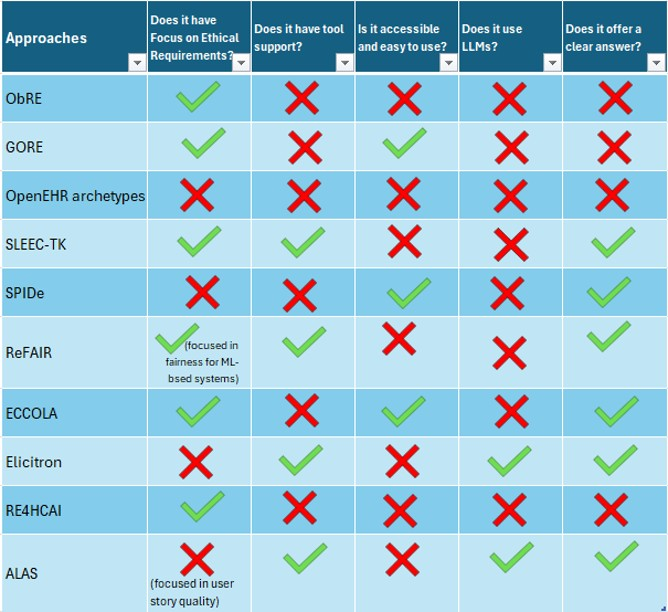
\includegraphics[width=0.8\textwidth]{state_of_the_art_results}
  \caption{State of the Art Research Results}
  \label{fig:state_of_the_art_results}
\end{figure}

% In conclusion, several studies examine approaches to elicit ethical requirements, but each method has its drawbacks. Ontology-based methods require input from experts and are not easily scalable. 
% Card-based and catalog methods, while practical, are static and may neglect emerging ethical concerns. AI-assisted techniques primarily focus on functional requirements and often need human refinement. 
% Our goal is to propose an approach that is more accessible and flexible, capable of adapting to evolving needs. This research aims to advance the field of ethical requirements by utilizing LLMs in 
% the requirement elicitation process.

\subsection{Summary}
In this chapter, we reviewed existing approaches for eliciting ethical requirements. We examined ontology-based frameworks, card-based methods, and agile techniques like Ethical User Stories. Additionally, we explored 
AI-assisted methods for requirements elicitation, such as agent-based simulations and LLM-driven user story refinement. Each approach was analyzed for its strengths and limitations, highlighting challenges related to 
scalability, adaptability, and automation. This analysis lays the groundwork for our proposed solution, which aims to address these gaps by utilizing AI to create a dynamic catalog of ethical user stories.


